\subsection{SVD as a geometrical interpretation}

And what was the advantage of the factorization then? In simple terms,
decomposing the function behind matrix $A$, as a sequence of three
simpler (easier to understand) transformations. Here the geometric
interpretation helps to complete the picture, as orthogonal (change of
basis) matrices do represent rigid transformation in space, that is,
they do not alter the lengths of vectors (hence, preserve
shapes). Strictly speaking, orthogonal matrices can be decomposed as a
rotation and a reflection; but for geometric intuition, is often
desirable to think in the rotation part only. \\

On the other hand, diagonal matrices are the simplest transformation
possible, they do not change the basis but just expand or contract the
coordinates along the axis given by the basis. Again, if we consider
the generic case of diagonal matrices, a negative element $D_{ii}$
would additional provoke a reflection in the axis $i$; but since the
SVD decomposition produces only positive elements on the diagonal, we
ignore this case and just think in terms of contractions or
expansions along the axes. \\

Armed with this geometrical insight, we can enhance our understanding
of the action of $A$ through the SVD decomposition, by associating to
the simpler operations the corresponding geometrical transformations.
The geometric visualization usually requires a couple of
simplifications: first of all, the dimensions of domain and codomain
must be reduced; as it is easier to visualize things in \R{2} or
\R{3}, than in an arbitrary \R{n}. Given two dimensions fit well in a
screen, let us pick $\R{n} = \R{m} = \R{2}$. \\

Secondly, we need to focus our attention in an specific set of
points (as visualizing the effect of a linear transformation against
``all'' vectors in space, even for \R{2}, is a quite abstract and
complex task). The usual procedure is to pick the vectors in the
unitary sphere in \R{2} (which contains in particular the columns of
$V$, as they are unit orthogonal vectors). \\

Let us proceed now: let the matrix $A$ be of
dimensions $2  \times 2$, the matrices $V$ and $U$ be formed
by unit column vectors $\{\vec{v_1},\vec{v_2}\}$ and $\{\vec{u_1},\vec{u_2}\}$,
respectively; and let matrix $\Sigma$ be $diag(\sigma_1,\sigma_2)$
such that $\sigma_1 > \sigma_2 > 0$. We will additionally assume that
$\sigma_1 > 1$ and $\sigma_2 < 1$, in order to allow them represent an
expansion and contraction, respectively. The previously described steps of
the SVD factorization, can be now augmented with the corresponding
geometrical transformations: \\

\begin{enumerate}
\item Start with unit sphere in \R{2}, with the unit vectors \vec{v_1}
  and \vec{v_2} living inside of it. 
\item Action of \trans{V}: Rotate the space such that \vec{v_1} and
  \vec{v_2} become the new orthogonal basis (this transformation
  leaves the shape of the sphere intact).
\item Action of $\Sigma$: Once rotated, the unit sphere is expanded
  in the direction of \vec{v_1} (per $\sigma_1$), and contracted in the
  direction of \vec{v_2} (per $\sigma_2$). 
\item Action of $U$: Once reshaped, the resulting ellipse is taken
  from the basis $\{u_1,u_2\}$ back to the canonical basis (this
  transformation changes the orientation of the ellipse, given that
  is not a symmetric figure; but still it preserves it shape).
\end{enumerate}
\hfill

These steps can be summarized in the following figure \footnote{Which
  was taken from a \href{http://math.stackexchange.com/questions/243811/visualization-of-singular-value-decomposition-of-a-symmetric-matrix}{MathStackExchange phorum post}, we
  could not locate back the original source though.}: \\

\begin{figure}[h]
  \centering
  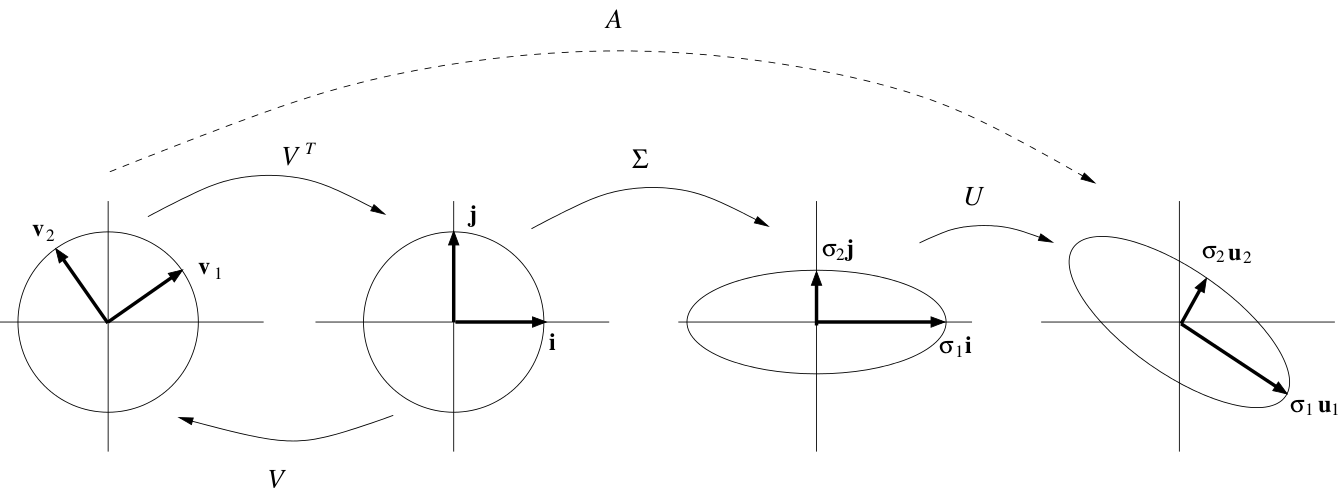
\includegraphics[width=15cm]{svd-geo-diag}
  \caption{Geometrical interpretation of $A = U \Sigma \trans{V}$,
    over the unit sphere.}
  \label{fig:svd-geo-diag}
\end{figure}
\hfill
